% !TEX root = Eco-Model.tex
\section{Design of the ecosystem} % (fold)
\label{sec:design_of_the_ecosystem}
\subsection{Preliminaries} % (fold)
\label{sub:preliminaries}
The manufacturing ecosystem we proposed in this paper consists of the structure of cloud manufacturing, the operation mode and the controlling rules. Before the detailed interpretation for these parts, we describe some basic settings as follows.

\subsubsection{Master plan} % (fold)
\label{ssub:master_plam}
With the cloud manufacturing platform operating, demander comes, signs up and publish orders. Match module in platform informs the task messages in the order to every matched resources and services. After the select decision makes by the demander, the selected resources and services prepare to the performance of the task.
Providers find frequent task after a bunch of successful accomplishment via resource reviews, then another type of job, service-call generated by them to gather certain type and amount of resources registered in the platform to create service in order to perform the certain task more efficient than before. Most of resource related decision making are well controlled by platform with the review module.

A single order($o_i$) consists of a set $\mathcal{T}_i = \left\{ t_{i1},t_{i2},\dots\right\}$ of tasks which have to be processed. The tasks are interrelated by kinds of constraints. First, precedence constraints force task $t_{ij}$ not to be started before all its immediate predecessors, how to construct the predecessor will be explained later. Second, performing the tasks requires resources with limited capacities. Third, resources cooperation transmits and enhances these constraints.

A single resource($mr_k$) belongs to one type in set $\mathcal{A} = \left\{1,2,\dots\right\}$ given by the platform. While being processed via resource cooperation, task $t_{ij}$ requires $q_{k,ij}$ units amount of the resources with every type in $\mathcal{A}_{ij}\subset\mathcal{A}$ during every period of its non-preemptable duration $p_{ij}$. Each resource $mr_k$ has a limited capacity of $C_k(\tau)$ at any point in time $\tau$.

A single service($s_l$) is a composition of all resources in set $R_l$ with their partial capacities, it can only process certain task with matched resource configuration($\mathcal{A}_{ij}=\mathcal{A}_l$,$ Q_{ij}(\cdot)=Q_l(\cdot)$) without resource coordinating any more. While being processed via one matched service, task can be suspended then outsourced to other matched service or resource cooperation.
Resource comes along with provider when it enter the ecosystem, however, service doesn't, service is generated after a period of time, the prototype of a service is another type of job, we call it the service-call.

A single service-call($sc_l$) comes out after the finish of one frequent task, so it have the same resource configuration the frequent task. Service-call can only be performed via resource cooperation with duration $p_l$, because the identity of resource, the capacity cannot be return to the resource after the finish of service-call, so the service-call brings new constrains to the related resources. Unlike the task, the amount of one type resource required in the service-call can be pieced together from more than one resource as long as they are in the same type.

Specifically, a simple instance with configuration \autoref{tab:simpleresourceconfiguration}--\ref{tab:simplejobconfiguration} and schedule chart \autoref{fig:scheduleChart} will describe the setting more clearly.
\begin{table}[htbp]
  \centering
  \scriptsize
  \caption{Simple resource configuration}
    \begin{tabular}{ccc}
    \toprule
    Resource & Type  & Capacity \\
    \midrule
    $r_1$ & 1     & 10 \\
    $r_2$ & 2     & 10 \\
    $r_3$ & 3     & 10 \\
    $r_4$ & 3     & 10 \\
    \bottomrule
    \end{tabular}%
  \label{tab:simpleresourceconfiguration}%
\end{table}%
\begin{table}[htbp]
  \centering
  \scriptsize
  \caption{Simple job configuration}
    \begin{tabular}{cccccc}
    \toprule
    \multicolumn{1}{c}{\multirow{2}[0]{*}{ Job}} & \multicolumn{3}{c}{Need Resource Capacity} & \multicolumn{1}{c}{\multirow{2}[0]{*}{Release Time}} & \multicolumn{1}{c}{\multirow{2}[0]{*}{Process Duration}} \\
    \multicolumn{1}{c}{} & $Type_1$ & $Type_2$ & $Type_3$ & \multicolumn{1}{c}{} & \multicolumn{1}{c}{} \\
    \midrule
    $t_1$ & 0     & 5     & 7     & 0     & 7 \\
    $t_2$ & 7     & 5     & 7     & 4     & 5 \\
    $t_3$ & 6     & 0     & 5     & 2     & 3 \\
    $sc_1$ & 0     & 0     & 3    & 1     & 1 \\
    $sc_2$ & 2     & 7     & 6     & 3     & 1 \\
    \bottomrule
    \end{tabular}%
  \label{tab:simplejobconfiguration}%
\end{table}%
\begin{figure}[htbp]
	\centering
	\resizebox{.8\textwidth}{!}{% !TEX root = flow_head.tex


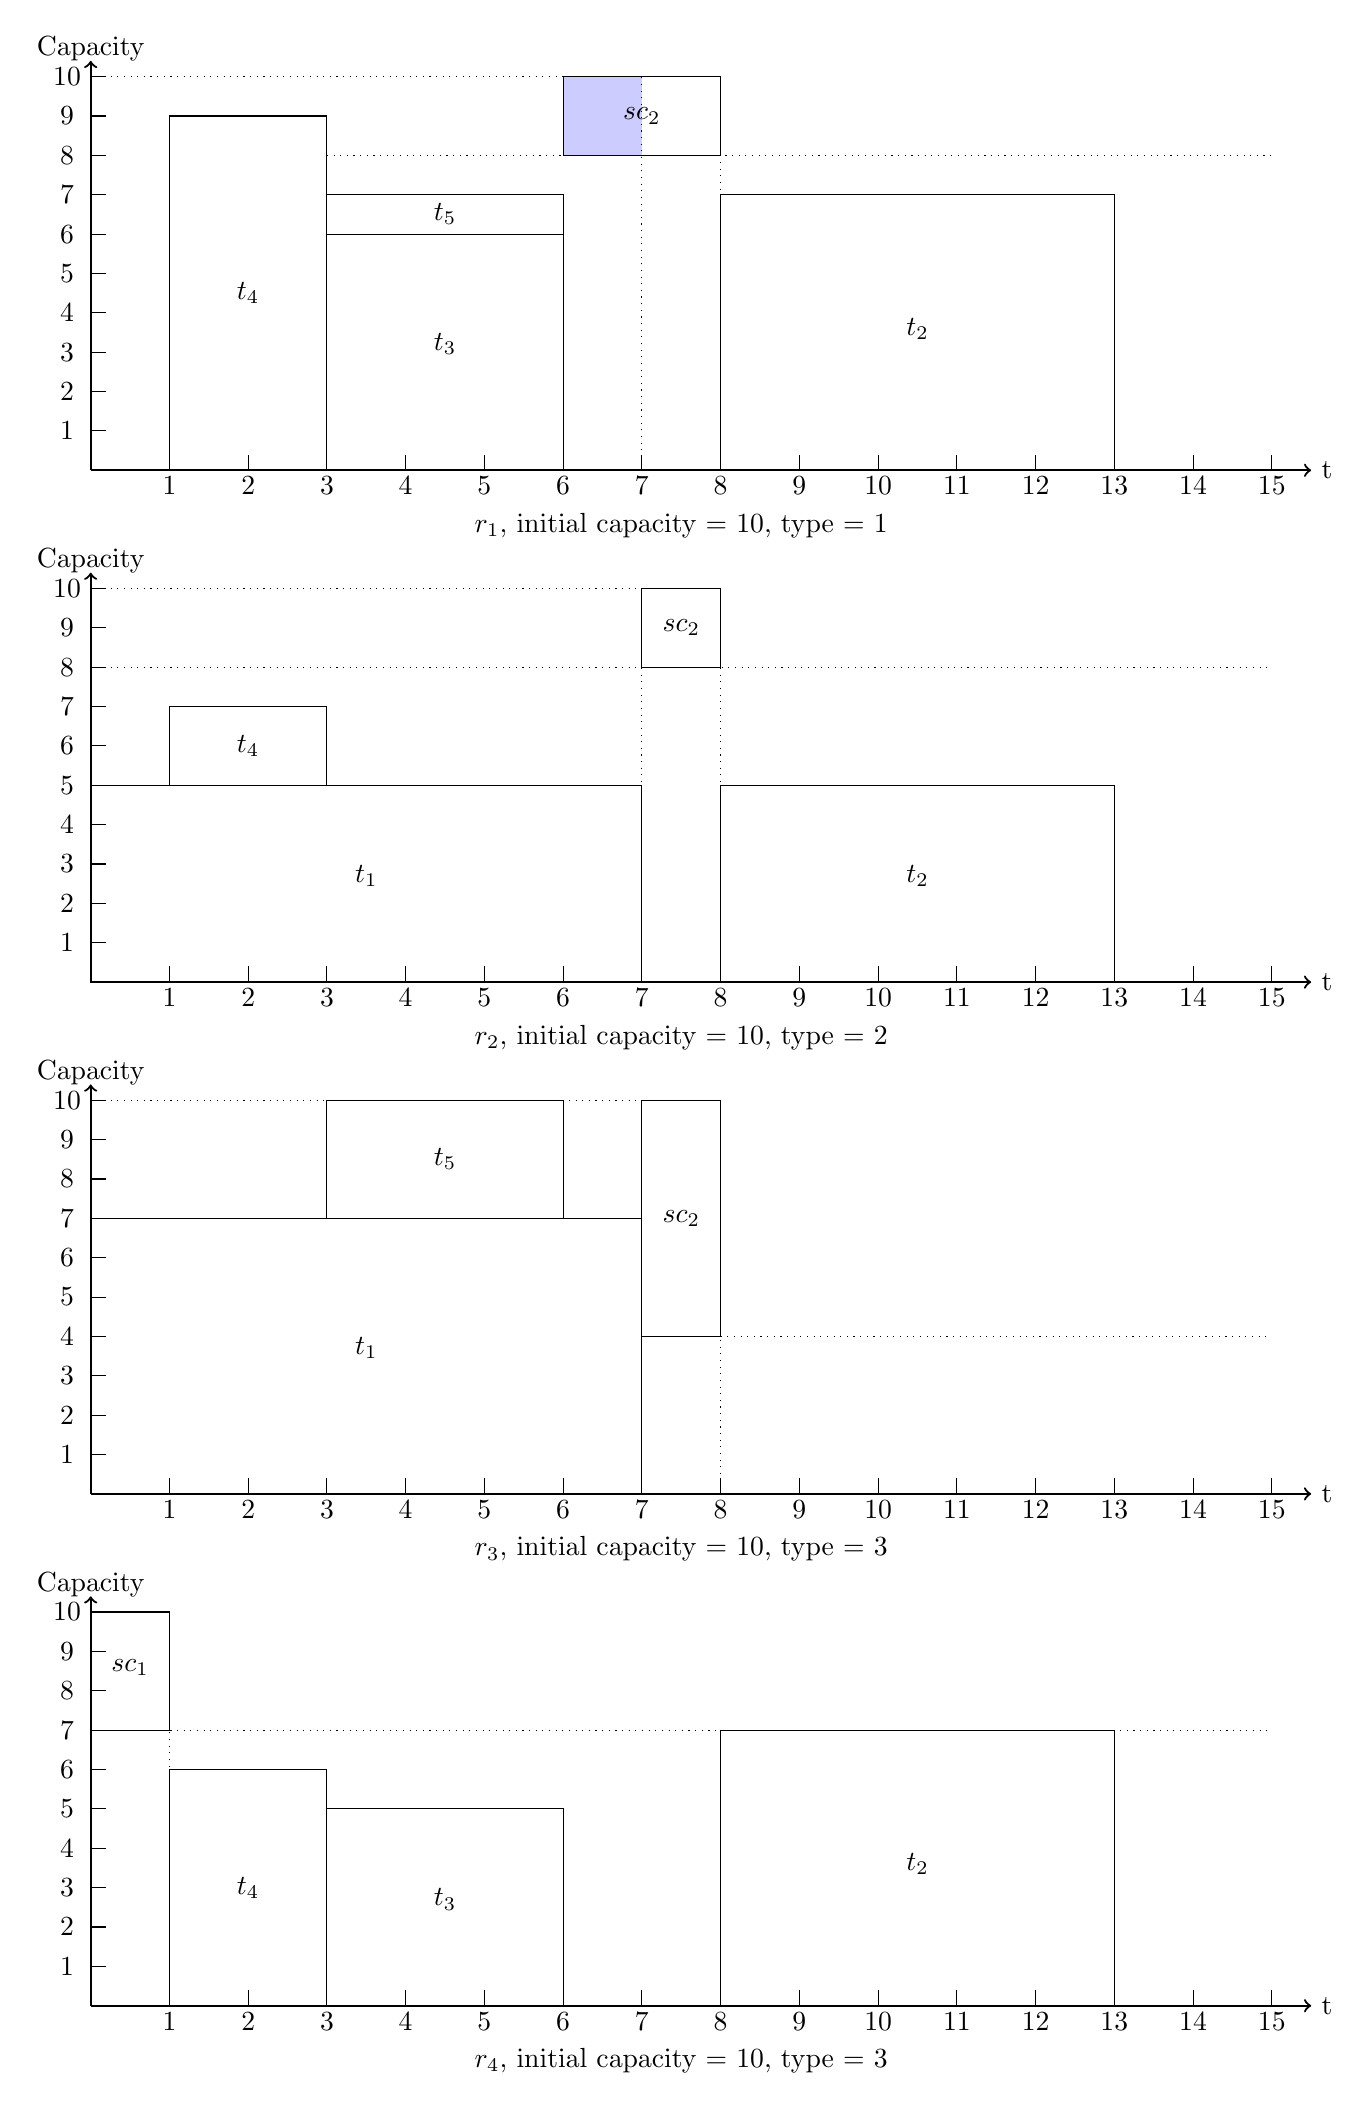
\begin{tikzpicture}
\foreach \x in {0,6.5,13,19.5}
	\draw [->,thick] (15.7cm,\x cm) node{t} (0,\x cm) -- +(15.5cm, 0) ;
\foreach \x in {0,6.5,13,19.5}
	\draw [->,thick] (0,\x cm) -- +(0,5.2 cm);
\foreach \x in {0,6.5,13,19.5}
	\draw[yshift=5.35cm] (0,\x cm) node{Capacity};
\foreach \x in {1,...,15}
	\foreach \y in {0,6.5,13,19.5}
		\draw (\x cm,\y cm) -- +(0,2mm);
\foreach \x in {1,...,15}
	\foreach \y in {0,6.5,13,19.5}
		\draw[yshift=-2mm] (\x cm,\y cm) node{$\x$};
\foreach \y in {0,6.5,13,19.5}
	\foreach \x in {1,...,10}
		\draw[yshift=\y cm] (0,0.5*\x cm) -- +(2mm,0) (-3mm,0.5*\x cm) node{$\x$};

\draw (7.5cm,-7mm) node{$r_4$, initial capacity = 10, type = 3};
\draw[yshift=6.5cm] (7.5cm,-7mm) node{$r_3$, initial capacity = 10, type = 3};
\draw[yshift=13cm] (7.5cm,-7mm) node{$r_2$, initial capacity = 10, type = 2};
\draw[yshift=19.5cm] (7.5cm,-7mm) node{$r_1$, initial capacity = 10, type = 1};

\fill[blue!20!,yshift=19.5cm] (6cm,4cm) rectangle (7cm,5cm);
\draw[yshift=19.5cm] (3cm,0) rectangle (6cm,3cm) (6cm,4cm) rectangle (8cm,5cm) (8cm,0) rectangle (13cm,3.5cm) (1cm,0) rectangle (3cm,4.5cm) (3cm,3cm) rectangle (6cm,3.5cm)  (4.5cm,1.6cm) node{$t_3$} (7cm,4.5cm) node{$sc_2$} (10.5cm,1.8cm) node{$t_2$} (2cm,2.25cm) node{$t_4$} (4.5cm,3.25cm) node{$t_5$};
\draw[dotted,yshift=19.5cm] (0,5cm) -- (7cm,5cm) (3cm,4cm) -- (15cm,4cm) (7cm,0) -- (7cm,5cm) (8cm,4cm) -- (8cm,3.5cm);
\draw[yshift=13cm] (0,0) rectangle (7cm,2.5cm) (7cm,4cm) rectangle (8cm,5cm) (8cm,0) rectangle (13cm,2.5cm) (1cm,2.5cm) rectangle (3cm,3.5cm)  (3.5cm,1.35cm) node{$t_1$} (7.5cm,4.5cm) node{$sc_2$} (10.5cm, 1.35cm) node{$t_2$}  (2cm,3cm) node{$t_4$};
\draw[dotted,yshift=13cm] (0,5cm) -- (7cm,5cm) (0,4cm) -- (15cm,4cm) (7cm,5cm) -- (7cm,0) (8cm,5cm) -- (8cm,0);
\draw[yshift=6.5cm] (0,0) rectangle (7cm,3.5cm) (7cm,2cm) rectangle (8cm,5cm) (3cm,3.5cm) rectangle (6cm,5cm) (3.5cm,1.85cm) node{$t_1$} (7.5cm,3.5cm) node{$sc_2$} (4.5cm,4.25cm) node{$t_5$};
\draw[dotted,yshift=6.5cm] (0,5cm) -- (7cm,5cm) (8cm,2cm) -- (15cm,2cm) (8cm,0) -- (8cm,2cm);
\draw (0,3.5cm) rectangle (1cm,5cm) (3cm,0) rectangle (6cm,2.5cm) (8cm,0) rectangle (13cm,3.5cm) (1cm,0) rectangle (3cm,3cm) (4.5cm, 1.35cm) node {$t_3$} (0.5cm,4.3cm) node{$sc_1$} (10.5cm,1.8cm) node{$t_2$} (2cm,1.5cm) node{$t_4$};
\draw[dotted] (0,3.5cm) -- (15cm,3.5cm) (1cm,0) -- (1cm,3.5cm);
\end{tikzpicture}
}
	\caption{Simple instance schedule chart with 4 resources}
	\label{fig:scheduleChart}
\end{figure}
This instance makes some simplification in the subscript fields in order to emphasize the resource cooperation, all the job(task and service-call) performance can only be started when the each of the related resource is ready, so the shadow in the figure is the waiting period. Horizontal dotted line constrained the available capacity of the resource for the following jobs, every performance of service-call will make the line lower and it will never get higher again unless the related service is repealed.

% subsubsection master_plan (end)

\subsubsection{Assumptions, nomenclature} % (fold)
\label{ssub:assumptions_nomenclature}
Assumptions about quality

about time

schedule and outsource are event driven decision making 

\begin{table}[!h]
\begin{tabularx}{\textwidth}{|lX|}
    \hline
    \multicolumn{2}{|l|}{\multirow{2}[0]{*}{\large\textbf{Nomencalture}}} \\
    \multicolumn{2}{|l|}{} \\
	$o_i$ & Order that come with demander \\
	$\mathcal{T}_i$ & Task set of $o_i$ \\
	$t_{ij}$ & Task belongs to $o_i$, $t_{ij}\in\mathcal{T}_i$ \\
	$p_{ij}$ & Process duration of $t_{ij}$\\
	$r_i$ & Release time of $o_i$\\
	$f_{ij}$ & Actual finish time of $t_{ij}$ \\
	$f_{i}$ & Finish time of $o_i$\\
	$\mathcal{P}_{ij}$ & The set of predecessor of $t_{ij}$\\
	$mr_k$ & Resource that come with provider \\
	$\delta_k$ & Quality of resource $mr_k$ \\
	$C_{k,\tau}$ & Capacity of $mr_k$ at time $\tau$\\
	$A_{k,\tau}$ & Available capacity of $mr_k$ at time $\tau$\\
	$\mathcal{L}_{k,\tau}$ & The list of job queue of $mr_k$ at $\tau$ with sequence\\
	$\mathcal{G}_{k,\tau}$ & The set of active job (being processed) of $mr_k$ at $\tau$ \\ 
	$f^{(s)}_j$ & Ideal finish time of $t_j$ in $\mathcal{L}^{(s)}_{k,\tau_0}$ for schedule . \\
	$re_j$ & Remaining process time of $t_j$ in $\mathcal{G}_{k,\tau_0}$ for schedule . \\
	$\mathcal{A}$ & Resource type set \\
	$\mathcal{A}_{ij}$ & Resource type subset required by $t_{ij}$, $\mathcal{A}_{ij}\subset\mathcal{A}$\\
	$q_{\alpha,ij}$ & Required amount of resource with type $\alpha$ by $t_{ij}$\\
	$sc_l$ & Service-call generated by provider\\
	$p_l$ & Process duration of $sc_l$\\
	$r_l$ & Release time of $sc_l$\\
	$\mathcal{P}_{l}$ & The set of predecessor of $sc_{l}$\\
	$\mathcal{A}_l$ & Resource type subset required and provided by $sc_l$ and $ms_l$ respectively, $\mathcal{A}_l\subset\mathcal{A}$\\
	$ms_l$ & Service that generated after the finish of $sc_l$\\
	$\Delta_l$ & Overall quality of servicev $ms_l$\\
	$\bm{mr}_l$ & Resource member set of $ms_l$\\
	$\bm{q}_l$ & Resource member's capacity contribution set of $ms_l$\\
	$\mathcal{L}_{l,\tau}$ & The list of job queue of $ms_l$ at $\tau$ with sequence\\
	$\mathcal{G}_{k,\tau}$ & The set of active job (being processed) of $ms_l$ at $\tau$ \\
	$\mathcal{R}_{ij,\tau}$ & Resource candidates set for $t_{ij}$ to select\\
	$\mathcal{B}_{ij,\tau}$ & Resource candidate types set for $t_{ij}$\\
	$\mathcal{S}_{ij,\tau}$ & Service candidates set for $t_{ij}$ to select\\
	$\mathcal{R}_{l,\tau}$ & Resource candidates set for $sc_l$ to select\\
	$\mathcal{B}_{l,\tau}$ & Resource candidate types set for $sc_l$\\
	$R(\cdot)$ & Rank inquire function about provider\\
	$F(\cdot)$ & Owner inquire function about resource or service\\
	$P(\cdot)$ & Type inquire function about resource\\
	$\bm{x}$ & Bold font of the variable($x$) means the temp set of a bunch of these variables\\
    \hline
\end{tabularx}
\end{table}

For the continuous coming of provider, demander, order, task, etc., the amount of them can not be determined at any time point, so we doesn't restrict the upper bound for subscript index amount of all these variables, and we will study the decision separately for these individual at the given time point $\tau$. Detailed design will be explained in the following sections.
% subsubsection assumptions_nomenclature (end)
% subsection preliminaries (end)

\subsection{Interactions and decisions} % (fold)
\label{sub:interactions_and_decisions}
\subsubsection{Demander}
\label{subs:Demander}
Demander makes decision about resources and services selection for the task. Without loss of generalization, we suppose at time period $\tau$, demander received bunch of matched resource and services as candidates for the performance of the published order $o_i$, it's obvious that $\tau \ge r_{i}$. The decision making for any task included in $o_i$, let's take $t_{ij}$, can be described in one of the following 3 situation:

\begin{asparaenum}
\item $\mathcal{B}_{ij,\tau}\subset\mathcal{A}_{ij}$, while $|\mathcal{S}_{ij,\tau}|>0$.
\suspend{asparaenum}
\begin{equation}
\max_{\forall l}\left( \Delta_{l}, R\left(F\left(ms_{l}\right)\right), \abs{\mathcal{L}_{l,\tau}}\right)
\end{equation}
\begin{numcases}{\text{s.t.}}
\Delta_l \sim \mathcal{N} \left(\mu_l,\sigma_l^2\right) & \\
\mu_l = mean\left( \bm{mr}_l , \bm{q}_l \right) & \\
\sigma_l = std\left( \bm{mr}_l , \bm{q}_l \right) & \\
l \in \left\{l' |  ms_{l'} \in \mathcal{S}_{ij,\tau} \right\}  & 
\end{numcases}

\resume{asparaenum}
\item  $\mathcal{B}_{ij,\tau} = \mathcal{A}_{ij}$, while $\abs{\mathcal{S}_{ij,\tau}}=0$.
\suspend{asparaenum}

\begin{equation}
\max_{\forall \bm{k}}\left( \delta_{\bm{k}}, 
R\left( F\left( mr_{\bm{k}} \right) \right), \abs{\mathcal{L}_{\bm{k},\tau} }
\right)
\end{equation}

\begin{numcases}{\text{s.t.}}
q_{\alpha,ij} \le C_{k_{\alpha},\tau} & $\alpha\in\mathcal{A}_{ij}$\\
R_{\alpha,\tau} = \left\{ mr| mr\in\mathcal{R}_{ij,\tau}, P(mr) = \alpha \right\} & $\alpha\in\mathcal{A}_{ij}$\\
\mathcal{R}_{ij,\tau} = \bigcup_{\alpha\in\mathcal{A}_{ij}}\mathcal{R}_{\alpha,\tau} & \\
\bm{k} = \left[k_1,\dots ,k_\alpha,\dots,k_{\abs{\mathcal{A}_{ij}}} \right] & \\
k_\alpha \in \left\{ k | mr_k \in \mathcal{R}_{\alpha,\tau} \right\} &$\alpha\in\mathcal{A}_{ij}$
\end{numcases}
For each required resource type $\alpha$

\resume{asparaenum}
\item  $\mathcal{B}_{ij,\tau} = \mathcal{A}_{ij}$, while $\abs{\mathcal{S}_{ij,\tau}}>0$.
\end{asparaenum}

\begin{gather}
\max_{m\in\{l^*,\bm{k}^*\}} \left( \Delta_m, 
Rank_m, \mathcal{L}_m \right) \\ 
\text{s.t.}\notag
\end{gather}
\begin{numcases}{}
q_{\alpha,ij} \le C_{k_{\alpha},\tau} & \footnotesize$\alpha\in\mathcal{A}_{ij}$\\
R_{\alpha,\tau} = \left\{ mr| mr\in\mathcal{R}_{ij,\tau}, P(mr) = \alpha \right\} & \footnotesize$\alpha\in\mathcal{A}_{ij}$\\
\mathcal{R}_{ij,\tau} = \bigcup_{\alpha\in\mathcal{A}_{ij}}\mathcal{R}_{\alpha,\tau} & \\
\bm{k} = \left[k_1,\dots ,k_\alpha,\dots,k_{\abs{\mathcal{A}_{ij}}} \right]& \\
k_\alpha \in \left\{ k | mr_k \in \mathcal{R}_{\alpha,\tau} \right\} &\footnotesize$\alpha\in\mathcal{A}_{ij}$ \\
\bm{k}^* = \arg\left(\max_{\forall \bm{k}}\left( \delta_{\bm{k}}, 
R\left( F\left( mr_{\bm{k}} \right) \right), \abs{\mathcal{L}_{\bm{k},\tau} }
\right)\right) & \\
Rank_{\bm{k}^*} = \min_{k\in\bm{k}^*} \left\{ R\left( F\left( mr_k \right) \right) \right\} & \\
\mathcal{L}_{\bm{k}^*} = \max_{k\in\bm{k}^*}\left\{ \abs{\mathcal{L}_{k,\tau}} \right\} & \\
\Delta_{\bm{k}^*} \sim \mathcal{N} \left(\mu_{\bm{k}^*},\sigma_{\bm{k}^*}^2\right) & \\
\mu_{\bm{k}^*} = mean\left( \bm{mr}_{\bm{k}^*} , \bm{q}_{\bm{k}^*} \right) & \\
\sigma_{\bm{k}^*} = std\left( \bm{mr}_{\bm{k}^*} , \bm{q}_{\bm{k}^*} \right) & \\
\bm{mr}_{\bm{k}^*} = \bigcup_{k\in\bm{k}^*}mr_k  &\\
\bm{q}_{\bm{k}^*}  =\bigcup_{\alpha\in\mathcal{A}_{ij}}q_{\alpha,ij} & \\
\Delta_l \sim \mathcal{N} \left(\mu_l,\sigma_l^2\right) & \\
\mu_l = mean\left( \bm{mr}_l , \bm{q}_l \right) & \\
\sigma_l = std\left( \bm{mr}_l , \bm{q}_l \right) & \\
l \in \left\{l' |  ms_{l'} \in \mathcal{S}_{ij,\tau} \right\}  & \\
l^* = \arg\left( \max_{\forall l}\left(\Delta_{l}, R\left(F\left(ms_{l}\right)\right), \abs{\mathcal{L}_{l,\tau}}\right)  \right) & \\
Rank_{l^*} = R\left( F\left( ms_{l^*} \right) \right) & \\
\mathcal{L}_{l^*} = \abs{\mathcal{L}_{l^*,\tau}} & \\
m \in \left\{ l^*,\bm{k}^* \right\}
\end{numcases}

\subsubsection{Provider}
\label{subs:Provider}
Provider makes decision for job response with regard to its resources and service, the job here is the generalization of task and service-call. As we mentioned in the master plan, provider publish service-call according to the frequent accomplished tasks. Without loss of generalization, we suppose at time $\tau$, demander will make these decisions:

\begin{asparaenum}
\item Response for the task need $t_{ij}$($\tau\ge r_i$) with resource $mr_k$
\suspend{asparaenum}
\begin{numcases}{}
A_{k,\tau} \ge q_{\alpha,ij} &\\
P(mr_k) = \alpha &
\end{numcases}
If $mr_k$ meets the above condition, provider of it will response the task need, demander of $t_{ij}$ will add $mr_k$ to $\mathcal{R}_{ij,\tau}$. If $mr_k$ was finally chose, available of $mr_k$ will change as $A_{k,\tau}:= A_{k,\tau} - q_{\alpha,ij}$. The available will be return back after the finish of $t_{ij}$.
\resume{asparaenum}
\item Response for the service-call need $sc_l$($\tau\ge r_l$) with resume $mr_k$
\suspend{asparaenum}
\begin{numcases}{}
C_{k,\tau} > 0 & \\
P(mr_k) = \alpha
\end{numcases}
If $mr_k$ meets the above condition, provider($p_a$) of it will response the service-call need, the provider($p_b$) of $sc_l$ will add $mr_k$ to $\mathcal{R}_{l,\tau}$, it's possible to let $p_a=p_b$. If $mr_k$ was finally chose, capacity of $mr_k$ will change as:
\begin{numcases}{}
C_{k,\tau} := C_{k,\tau} - q_{\alpha,l}& If $C_{k,\tau} \ge q_{\alpha,l}$\\
C_{k,\tau} := 0 & otherwise
\end{numcases}

Capacity will not return back to $mr_k$ until the corresponding service $ms_l$ was repealed. Decision making of provider $p_b$ likes the one of demander's, but the final decision $\bm{mr}_l$ and $\bm{q}_l$ don't have to meet $\abs{\bm{mr}_l} = \abs{\mathcal{A}_{ij}}$, because different resource with the same type can gather together to bundle into one service, the only condition in need is that
\begin{numcases}{}
\sum_{k\in\mathcal{R}_{\alpha,\tau}} q_{\alpha,k} = q_{\alpha,l} & $\forall\alpha\in\mathcal{A}_l$\\
R_{\alpha,\tau} = \left\{ mr| mr\in\mathcal{R}_{l,\tau}, P(mr) = \alpha \right\} & $\forall\alpha\in\mathcal{A}_l$
\end{numcases}
\resume{asparaenum}
\item Response for the task need $t_{ij}$($\tau\ge r_i$) with service $ms_l$.
\end{asparaenum}
Service is a combination contract among the participated resources and it's made oriented to the certain task, so the only condition for $ms_l$ to response $t_{ij}$ is:
\begin{numcases}{}
q_{\alpha,ij} = q_{\alpha,l} & $\forall\alpha\in\mathcal{B}_l$\\
\mathcal{A}_{ij} = \mathcal{B}_l
\end{numcases}

This condition is much same as service-call need $sc_l$ after the accomplishment frequent task $t_{ij}$:
\begin{numcases}{}
q_{\alpha,ij} = q_{\alpha,l} & $\forall\alpha\in\mathcal{A}_l$\\
\mathcal{A}_{ij} = \mathcal{A}_l
\end{numcases}
% subsection interactions_and_decisions (end)

\subsection{Operation mode} % (fold)
\label{sub:operation_mode}
The chief decision making about operation mode for provider is the job schedule method outsource mode, as we mentioned in the master plan, provider makes these decision to arrange the job for a better performance in the process procedure. Because of the event driven assumptions, we again suppose that both a new task was assigned to service or resource and a job was finished at time $\tau$, provider will make decision in the following conditions:
\begin{asparaenum}
\item Assign new task $t_{ij}$ in $mr_k$.
\suspend{asparaenum}

With the select decision of $t_{ij}$ to assign on $mr_k$ at $\tau$, the first thing for the provider of $mr_k$ is to set the predecessor set:
\begin{equation}
	\mathcal{P}_{ij} := \mathcal{P}_{ij}\cup \left\{ sc| sc\in\mathcal{L}_{k,\tau},sc \text{ is service-call} \right\} \cup \mathcal{G}_{k,\tau}
\end{equation}
Then, the provider will add $t_{ij}$ to queue or process buffer according to:
\begin{numcases}{}
\mathcal{G}_{k,\tau} := \mathcal{G}_{k,\tau} \cup \{t_{ij}\} & if $\abs{\mathcal{L}_{k,\tau}}=0$ and $A_{k,\tau}\ge q_{\alpha,ij}$ \\
\mathcal{L}_{k,\tau} := \mathcal{L}_{k,\tau} \cup \{t_{ij}\} & otherwise
\end{numcases}

\resume{asparaenum}
\item Assign new service-call $sc_l$ in $mr_k$.
\suspend{asparaenum}

With the select decision of $sc_l$ to assign on $mr_k$ at $\tau$, the first thing for the provider of $mr_k$ is to set the predecessor set:
\begin{equation}
	\mathcal{P}_l := \mathcal{P}_l\cup \mathcal{L}_{k,\tau} \cup \mathcal{G}_{k,\tau}
\end{equation}
Then, the provider will add $sc_l$ to queue or process buffer according to:
\begin{numcases}{}
\mathcal{G}_{k,\tau} := \mathcal{G}_{k,\tau} \cup \{sc_l\} & if $\abs{\mathcal{L}_{k,\tau}\cup\mathcal{G}_{k,\tau}}=0$ \\
\mathcal{L}_{k,\tau} := \mathcal{L}_{k,\tau} \cup \{t_{ij}\} & otherwise
\end{numcases}

\resume{asparaenum}
\item Schedule the tasks in $\mathcal{L}_{k,\tau}$.
\suspend{asparaenum}

The assignment of new service-call will not driven these decision making event because of the resource capacity consuming feature, so it's necessary to suspend service-call in inactive status until all the job before it in $\mathcal{L}_{k,\tau}$ are finished, at the meantime, all the job come after service-call should be stay in inactive status until the service-call is finished, as shown in \autoref{fig:simplejoblist}, service-call likes partition plate in $\mathcal{L}_{k,\tau}$.  
\begin{figure}[htbp]
	\centering
	\resizebox{.8\textwidth}{!}{% !TEX root = flow_head.tex
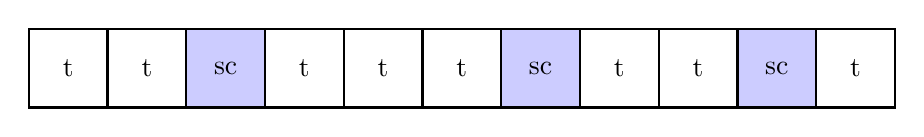
\begin{tikzpicture}

\foreach \x in {2,6,9}
	\fill[blue!20!] (\x cm, 0) rectangle +(1cm, 1cm);
\foreach \x in {2,6,9}
	\draw[xshift=.5cm] (\x cm,0.5cm) node{sc};	
\foreach \x in {0,...,10}
	\draw [thick] (\x cm, 0) rectangle +(1cm, 1cm);
\foreach \x in {0,1,3,4,5,7,8,10}
	\draw[xshift=0.5cm] (\x cm, 0.5cm) node{t};

\end{tikzpicture}
}
	\caption{Simple illustration for one $\mathcal{L}_{k,\tau}$}
	\label{fig:simplejoblist}
\end{figure}
Therefore, the we just need to schedule the tasks before the first service-call in $\mathcal{L}_{k,\tau}$ when one of the active job in $\mathcal{G}_{k,\tau}$ was finished at $\tau_0$, we denote the set of schedule task at this time as $\mathcal{L}^{(s)}_{k,\tau_0}$

A schedule is given by a vector of ideal finish times $\bm{f}^{(s)} = \left[f_1^{(s)}, f_2^{(s)},\dots,f^{s}_n\right],n=\abs{\mathcal{L}^{(s)}_{k,\tau_0}}$. Since the task in $\mathcal{L}^{(s)}_{k,\tau_0}$ and $\mathcal{G}_{k,\tau_0}$ may come from different orders, we here use the single uniform subscript $j$ to distinguish these tasks and their related variables, type subscript $\alpha$ can be ignored for all the job assigned here matches the resource type, so the schedule model is:

\begin{equation}
\min_{\forall\bm{f}^{(s)}}\left( \max_{j\in L^{(s)}}\left\{ f_j^{(s)} - r_j - p_j \right\} \right)
\end{equation}
\begin{numcases}{\text{s.t.}}
L^{(s)} = \left\{j| t_{j}\in \mathcal{L}^{(s)}_{k,\tau_0}\right\} & \\
f^{(s)}_h \le f_j^{(s)} - p_j & $h\in\mathcal{P}_j$,$j\in L^{(s)}$\\
G^{(s)} = \left\{j' | t_{j'}\in \mathcal{G}_{k,\tau_0}\right\} & \\
f^{(s)}_j =  \tau_0 + re_j & $j\in G^{(s)}$ \\
\sum_{j\in\left\{  j' |t_{j'} \in\mathcal{G}_{k,\tau}\right\}} q_j \le A_{k,\tau}& $\tau \ge \tau_0$ \\
% \bm{f}^{(s)} = \left[f_1^{(s)}, f_2^{(s)},\dots,f^{s}_{\abs{\mathcal{L}^{(s)}_{k,\tau_0}}}\right] & \\
f^{(s)}_j \ge \tau_0 + p_j & $j\in L^{(s)}$
\end{numcases}
\resume{asparaenum}
\item Schedule the task in $\mathcal{L}_{l,\tau}$
\suspend{asparaenum}



\resume{asparaenum}
\item Outsource the task in $\mathcal{L}_{l,
\tau}$ and $\mathcal{P}_{l,\tau}$
\end{asparaenum}


% subsection operation_mode (end)

\subsection{Controlling rules} % (fold)
\label{sub:controlling_rules}
Platform control the provider by the rank value and the review module
% subsection controlling_rules (end)

\subsection{Tricky problems} % (fold)
\label{sub:tricky_problems}
The job lock

add predecessor job when sc in to job queue,

after the finish of all the job in job queue to start the performance of sc

make the task which was prepared in one resource ahead to other jobs in the cooperated resources 
% subsection tricky_problems (end)
% section design_of_the_ecosystem (end)
